\section{Simulation studies}
\label{sec:sim}

The latent process is the scalar Ornstein--Uhlenbeck diffusion in Section~5.1 of \citet{golightly2026},
\[
\mathrm{d}X_t = \theta_1(\theta_2 - X_t)\,\mathrm{d}t + \theta_3\,\mathrm{d}W_t,
\]
with the Gaussian transition printed there. The truth is \(\theta = (1, 2, 1)\), the initial condition is \(x_0 = 10\), and observations at times \(1, \ldots, 16\) use \eqref{eq:obs} with \(H = 1\) and \(R = 0.1\). The prior is independent, \(\theta_1 \sim \mathrm{Gamma}(2, 2)\), \(\theta_2 \sim \mathrm{Gamma}(5, 3)\) and \(\theta_3 \sim \mathrm{Gamma}(2, 5)\), in the shape-rate parameterisation. The PDF writes \(\mathrm{Gamma}(a, b)\) without naming the parameterisation. We use shape and rate.

The nested filter uses \(M = 60\), \(N = 12\), \(\gamma = 0.4\) and \(k = 3\). The ensemble size does not adapt. Four replicate series are used. The gold standard for each series is a random-walk Metropolis--Hastings chain on \(\log\theta\), targeting the exact Kalman likelihood, with 3000 iterations after 1000 burn-in and proposal standard deviation 0.15. That chain is much shorter than the \(10^{6}\) iterations used by \citet{golightly2026}, and \(M\), \(T\) and \(N\) are smaller than in their Section~5.1. Posterior means from the pilot must be read with that Monte Carlo error in mind.

The reported error is the absolute difference, averaged over the three coordinates, between the weighted mean of \(\log\theta_i\) and the gold-standard mean. Cost is the number of transition draws. Tables~\ref{tab:s2}--\ref{tab:s6} give means over the four replicates. The files in the accompanying results directory contain the replicates.

\begin{table}[t]
\centering
\caption{Kernel comparison. Means over four replicates. Cost per acceptance is the number of rejuvenation transition draws divided by the number of accepted proposals. Source: \texttt{summary-s2.csv}.}
\label{tab:s2}
\begin{tabular}{lrrrr}
\hline
Kernel & Abs.\ error & Draws & Cost per acceptance & ESS \\
\hline
Metropolis--Hastings & 0.172 & 33855 & 310.4 & 39.6 \\
Delayed acceptance & 0.126 & 23970 & 221.6 & 43.3 \\
Switch at \(t = 8\) & 0.132 & 23457 & 214.7 & 36.7 \\
\hline
\end{tabular}
\end{table}

On the pre-registered criterion the switch is the best of the three kernels. Delayed acceptance is close to it and better than the plain random walk. The neighbour sets from the list and the tree agreed on all 491 checks per replicate on average. The list evaluated a distance to 29460 stored points on average and the tree to 13422.5. The agreement is the result that keeps the kernel unchanged. The distance count favours the tree at this size and does not include the cost of building the tree.

\begin{figure}[t]
\centering
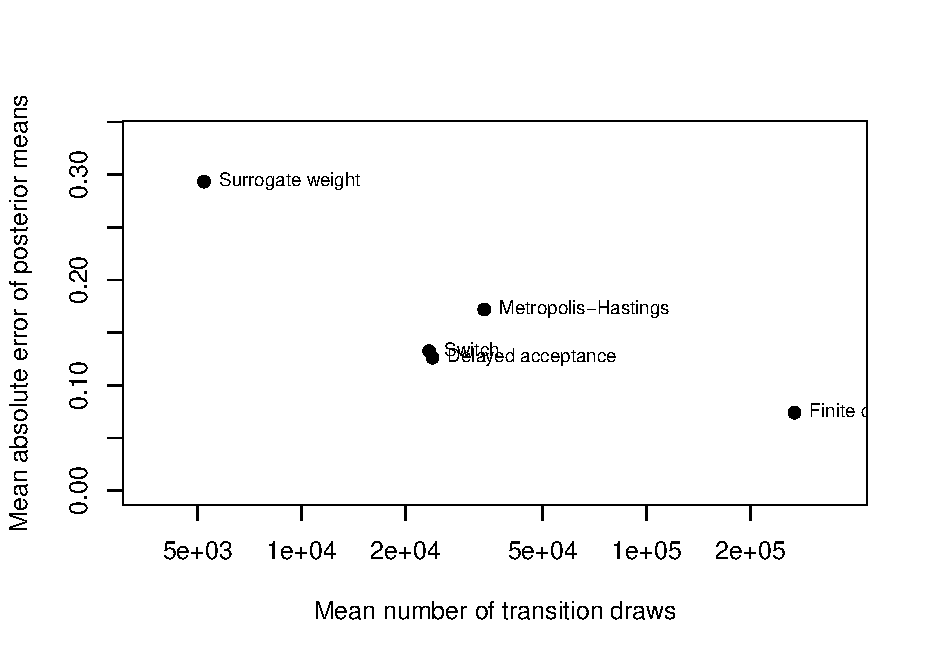
\includegraphics[width=0.85\textwidth]{figures/cost-error.pdf}
\caption{Mean absolute error of the posterior means of \(\log\theta_i\) against the mean number of transition draws. The finite-difference proposal is shown as a comparison that is not retained. Source: \texttt{summary-s2.csv}, \texttt{summary-s3.csv} and \texttt{summary-s4.csv}.}
\label{fig:cost}
\end{figure}

Figure~\ref{fig:cost} places the same runs on one scale, together with the surrogate-weight filter and the finite-difference proposal. The finite-difference proposal had mean absolute error 0.074 and mean transition draws 268602, against 0.172 and 33855 for the random walk. Effective sample size per transition draw was 0.000148 against 0.00123. The proposal does not improve that ratio. We do not retain it. The acceptance probability included the Gaussian proposal density, so the negative result is about cost, not about leaving \(\hat{\pi}_{\mathrm{enkf}}\).

The surrogate-weight filter used 5217 transition draws on average. The mean of the median absolute log differences between the surrogate increment and a fresh ensemble Kalman increment was 0.277, below the threshold of 1. The mean absolute error was 0.293, larger than the error of the plain filter and of delayed acceptance. The cost falls because most particles do not run a forecast. The target is \eqref{eq:knn-target}. The larger error is the visible part of the second approximation.

\begin{table}[t]
\centering
\caption{Sample variance of the log ensemble Kalman likelihood at the true parameter, from 20 independent ensembles. Source: \texttt{s5-variance.csv}.}
\label{tab:s5}
\begin{tabular}{rrrr}
\hline
\(d_y\) & \(N\) & Variance & Mean draws \\
\hline
1 & 8 & 14.060 & 128 \\
1 & 16 & 2.879 & 256 \\
5 & 8 & 24.935 & 640 \\
5 & 16 & 10.661 & 1280 \\
\hline
\end{tabular}
\end{table}

Table~\ref{tab:s5} is the scaling check that this pilot can support. The five-dimensional series is five independent copies of the same diffusion, with independent observation noise. Doubling \(N\) reduces the variance in both rows. The variance does not scale by the ratio of the observation dimensions. \citet[Proposition~2]{katzfuss2018} assumes independent draws from the true forecast in a different example. The ensemble used here is interacting, and the log-likelihood is a sum over the series. We do not draw a boundary at parameter dimension 10 or observation dimension 10.

\begin{table}[t]
\centering
\caption{Rao-Blackwellised weights. The identity row uses \(R_g = R = 0.1\). The other two rows use \(R_g = 0.5\) whilst the data and the gold standard use \(R = 0.1\). Error per draw is the ratio of the two means. Source: \texttt{summary-s6.csv} and \texttt{s6-identity.csv}.}
\label{tab:s6}
\begin{tabular}{lrrr}
\hline
Filter & Abs.\ error & Draws & Error per draw \\
\hline
Plain, \(R_g = 0.5\) & 0.369 & 22776 & \(1.62 \times 10^{-5}\) \\
Rao-Blackwellised, \(R_g = 0.5\) & 0.169 & 36069 & \(4.68 \times 10^{-6}\) \\
Rao-Blackwellised, \(R_g = 0.1\) & 0.121 & 31248 & \(3.87 \times 10^{-6}\) \\
\hline
\end{tabular}
\end{table}

When \(R_g = R\), the maximum absolute difference between the log ensemble Kalman increment and the log Rao-Blackwellised increment was 0 on each replicate. The correction does not change the weight. When \(R_g = 0.5\) and the true observation variance is 0.1, both densities are Gaussian and \(f \ne g\). The Rao-Blackwellised filter then has the smaller error per draw. That comparison is not a nonlinear observation model, and SMC2 was not run.
